\begin{figure}[h]
	\begin{center}
  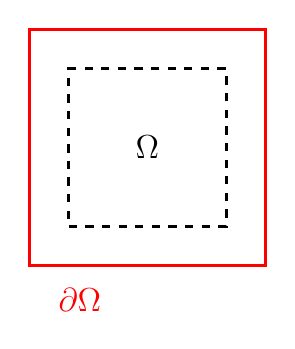
\begin{tikzpicture}[scale=0.5]
    \tikzstyle{every node}=[font=\tiny]
    \draw[style=very thick, color=red] (0,0) node[fill=none, below
      right=1ex,color=red ] { { \large $\partial\Omega$ } } -- (6,0) -- (6,6) --
      (0,6) -- cycle;
    \draw[style=very thick,dashed] (1,1) -- (5,1) -- (5,5) -- (1,5) -- cycle;

    \draw (3,3) node[fill=none] { {\large $\Omega$} };
  \end{tikzpicture}
	\end{center}
  \caption{Eliminated Boundary Nodes}
	\label{fig:ReducedBCs}
\end{figure}
